\section{Motivating Applications}

As the prices and sizes of sensors drop, there has been a dramatic increase in
the production of timeseries data. Streams of timeseries data, represented as
sets of \texttt{<time, value>} pairs, can give applications insights into the
instantaneous or historical behavior of the physical world.  However, these
streams of data are only as useful as their contextual information.  This
contextual information, or \emph{metadata}, contains all data that describes a
stream, often including at least one of the following:

\begin{itemize}
\item a unique identifier (UUID)
\item timezone for the stream's timestamps
\item engineering units for the stream's values
\item the unit of time or sampling rate
\item location (building, floor, room, orientation, etc)
\item calibration constants
\item software versions
\end{itemize}

There has already been substantial research on the application of physical
timeseries data for electric vehicle charging~\cite{sortomme2011optimal},
electric grids~\cite{carreras2004evidence}, building
occupancy~\cite{richardson2008high} and fault
detection~\cite{fontugne2013strip}. Common to all of these applications of
timeseries data is the tacet assumption that a data stream, once identified or
discovered, will retain consistent metadata. For some circumstances, this
assumption is valid, but in the domain of physical timeseries data (often
produced by sensors), this is often not the case. Metadata can change due to
changes in location or orientation, repairing configuration error, or changes
in the deployment site or environment.
% need to be more clear on what those circumstances are, exactly. this is linked
% to the identity of timeseries streams

Current applications, telemetry platforms and time series databases do not
account for the inevitable evolutions in metadata for the streams they operate
on. Here, we describe a family of applications that require the ability to
perform queries at instantaneous moments in the past or over ranges over time.
These applications fall into three categories, each of which places its
own requirements on the underlying metadata storage and retrieval system:
offline analysis of timeseries data, analysis of metadata, and real-time
metadata-based streaming.

\if 0
For each of these, we want to list what the possible applications are,
the kinds of queries they will require, the functionality that they require,
and why current solutions do not make this easy. also maybe have a figure
on what these queries would look like, and maybe talk about how they aren't possible
without temporal data.
\fi

\subsection{Timeseries Analysis} \label{subsection:timeseriesanalysis}

Without a temporal dimension, metadata describing a timeseries can only
capture a single static context, which may not be consistent over the
whole timeseries. Adding duration to metadata means there is no invalidation
of prior data when metadata does change, enabling downstream consumers
of the timeseries data to make use more fine-grained descriptions.

There are two sample timeseries analysis applications we discuss here: 1) an
application that computes the average monthly energy usage for a building that
must account for a calibration correction partway through data collection, and
2) a anomaly detection application that wants to ``tag'' anomaly ranges of
timeseries data.

The first application may operate by pulling energy usage over a full year,
and then bucket the data by each month and compute the average. The calibration
constant represents the correction of errors in the measurement process. In Figure~\ref{fig:calibrationconstant},
the plot represents the measured energy after a calibration transformation is applied: at time $t_0$, the constant
is $1.1$ and at time $t_1$ the constant is corrected to be $1.5$. Precluding the recalculation and replacement
of the data in $[t_0, t_1]$, a consumer must be able to map ranges of timeseries data to the correct
constant. In systems that do not maintain the history of metadata associated with timeseries, a consumer would
see the constant as it existed either at $t_0$ or at $t_2$, resulting in an incorrect interpretation of the data.

\begin{figure}
\centering
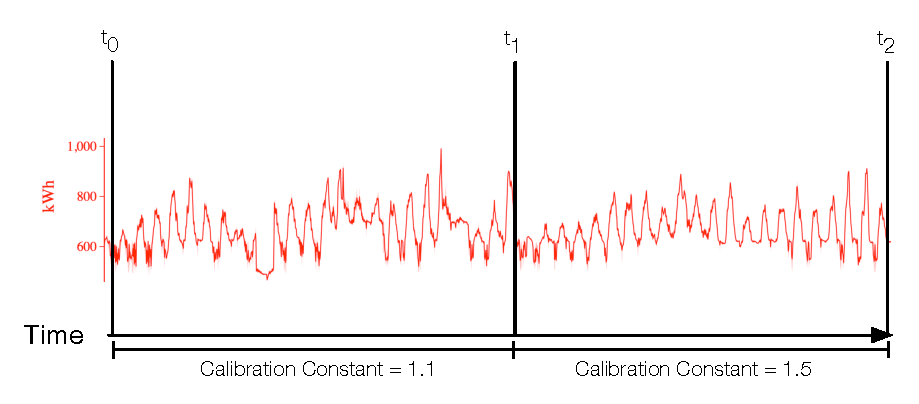
\includegraphics[width=.9\linewidth]{figs/calibrationconstant.pdf}
\caption{The calibration constant for the power meter timeseries changes and is reflected
in the metadata}
\label{fig:calibrationconstant}
\end{figure}

% how does the app work? describe the process. describe the metadata *and* data queries it wants. describe what would happen if it didn't have the metadata queries

The second application applies a set of heuristics to find anomalous events in a range of data; for example, data
in the range $[t_0, t_1]$ in Figure~\ref{fig:faultdetected}. This time range is ``tagged'' as anomalous in the metadata
for the stream. The benefit of storing this information in-band with other metadata rather than in an application-specific
store is that it becomes trivial for further consumers of this data to make more informed decisions about how to treat
that range of data.

\begin{figure}
\centering
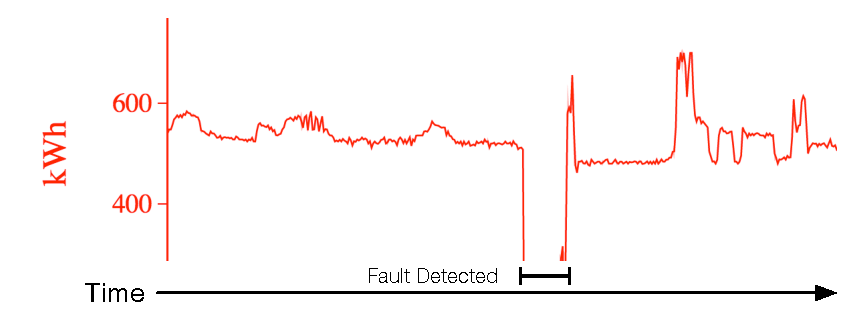
\includegraphics[width=.9\linewidth]{figs/faultdetected.pdf}
\caption{A range of data is tagged as unusual, warranting further investigation}
\label{fig:faultdetected}
\end{figure}

In both applications, the benefits of temporal metadata are clear: it guarantees
correctness and ``freshness'' on descriptions of timeseries data and provides
discoverable annotations of timeseries data that can be generated and shared across
consumers.

\if 0
Figure here: show some timeseries data (maybe a building feed w/ a configuration
constant change?). App needs to know to correct the data.

another figure: a temperature sensor moving from room to room?
figure: a plugstrip where what is plugged into it changes
\fi

\if 0
have some figure here,
- list of applications:
    - sensor move (floor, room, orientation, timezone)
    - software hanges
    - reporting rates change
    - calibration constants change
    - tagging of transient events: [T1, T2] was a voltage sag

Two benefits:
1. you know that the tags are correct and not just changed
2. you can tag events that you discover!
\fi

\subsection{Metadata Analysis}

Temporal metadata can also be used as a timeseries itself. Sensor timeseries,
or other data streams attached to physical objects, may experience changes in
location or orientation over the course of reporting. Maintaining a history of
these changes allows applications to ask questions such as ``which rooms did
this CO2 sensor sample from over the past month?'' or ``at time $t$, which
temperature sensors had a northern exposure?''. Another consumer may wish to
perform a frequency analysis on the anomalous events detected by the
application described in Section~\ref{subsection:timeseriesanalysis}, which
could involve retrieving the history of all anomaly tags applied to a
collection of streams. This may also include extracting the duration of these
anomalies, which can be derived from the ``start'' and ``end'' time of each of
the anomaly tags ($t_0$ and $t_1$ in Figure~\ref{fig:faultdetected}).

While these sorts of queries can be satisfied by storing attributes such as
room, orientation or exposure as distinct timeseries, this incorrectly treats
facts such as \texttt{Location/Room = 410 @ time $t_0$} as discrete data points
rather than continuous events. Note that this approach also does not remove the
need for metadata, as there must exist some mapping between a data timeseries
and its location timeseries.  Furthermore, the separation of metadata into
distinct timeseries can complicate basic queries: any metadata predicate that
involves multiple tags (e.g. \texttt{Location/Room},
\texttt{Sensor/Orientation} and \texttt{Sensor/SoftwareVersion}) involves
querying across as many timeseries.

%- treat metadata as data
%    - all rooms a sensor was in over past month
%    - all sensors that were in room XYZ at the time this event happened
%    - the fault detection app from above, but it wants to look at the history of detected faults
\subsection{Real-Time}

While beyond the current scope of this work, there is a family of real-time
applications that can be facilitated by materializing continuous views over a
collection of streams of timeseries data.

\begin{itemize}
\item control process takes avg temperature of all sensors in rooms 1,2,3
\item make a little figure for this?
\end{itemize}

%Motivating Applications
%- realtime change monitoring
%    - control process takes average of all sensors in rooms 1,2,3
